\documentclass[
    10pt,
    a4paper,
    % listof = totoc
]{scrartcl}
\usepackage{ucs}
\usepackage[utf8x]{inputenc}
\usepackage[english,ngerman]{babel}
\selectlanguage{ngerman}
\usepackage[T1]{fontenc}

% Math stuff
\usepackage{amsmath}
\usepackage{amsfonts}
\usepackage{amssymb}

% Farben
\usepackage[usenames,x11names,dvipsnames,rgb]{xcolor}
\definecolor{grey}{rgb}{0.4,0.4,0.4}
\definecolor{lightgrey}{rgb}{0.8,0.8,0.8}
\definecolor{ultralightgrey}{rgb}{0.96,0.96,0.96}

% Grafix
\usepackage{graphicx}

% Schriften
\usepackage{mathpazo,avant,courier}

% TikZ (dot2tex etc.)
% \usepackage{tikz}
% \usetikzlibrary{decorations, arrows, shapes}

% Farben in Tabellen
\usepackage{colortbl}

% Lange Tabellen
\usepackage{longtable}

% Gewrappte boxen (können innerhalb f{rame}box's verwendet werden)
\usepackage{minibox}

% FloatBarrier stellt z.B. sicher, dass das Literaturverzeichnis am Ende des
% Dokuments erscheint.
\usepackage{placeins}

% Hyperref
\usepackage{hyperref}
% Hypersetup
\hypersetup{
    pdftitle = {ES-HH - Software Design ras-weather},
    pdfauthor = {David Daniel},
    pdfsubject = {Software Design ras-weather},
    pdfkeywords = {Software Design} {ES-HH},
    % hidelinks
    colorlinks = true,
    linkcolor = blue,
    % urlcolor = black
    urlcolor = Blue,
    citecolor = grey
}
\urlstyle{same}

% Apa cite style
\usepackage{apacite}

% Glossar (load _after_ ! hyperref)
% \usepackage[toc]{glossaries}
% \makeglossaries
% \newglossaryentry{RTTI}
% {
    % name = {RTTI},
    % description = {"``Run time type information"'' liefert Informationen über
    % benutzerdefinierte Typen zur Laufzeit}
% }

% Listings
% @see http://tex.stackexchange.com/questions/51867/koma-warning-about-toc
% \usepackage{scrhack}
% \usepackage{listings}
% \lstset{
    % breakatwhitespace=true,
    % columns=fullflexible,
    % keepspaces=true,
    % breaklines=true,
    % tabsize=4, 
    % showstringspaces=false,
    % extendedchars=true,
    % basicstyle=\footnotesize\ttfamily,
    % numbers=left,
    % numberstyle=\scriptsize,
    % firstnumber=1
% }
% \lstdefinestyle{custom}{
    % belowcaptionskip=1\baselineskip,
    % captionpos = b,
    % breaklines=true,
    % frame=l,
    % xleftmargin=\parindent,
    % showstringspaces=false,
    % keywordstyle=\bfseries\color{green!40!black},
    % commentstyle=\itshape\color{purple!40!black},
    % identifierstyle=\color{blue},
    % stringstyle=\color{orange},
% }

\title{ES-HH - Software Design}
% \subtitle{}
\author{Andreas Hasler \\{\small andreas.hasler@students.ffhs.ch}
\and David Daniel\\{\small david.daniel@students.ffhs.ch}}
\date{\today}

\begin{document}
\maketitle
\pagenumbering{Alph}% Use uppercase alphabetic page numbers (and reset to A)

\begin{abstract}
    Dieses Dokument erläutert die Architektur Überlegungen zum Software Design für
    ras-weather. Die hier diskutierte Architektur bezieht sich auf die Software, welche
    auf dem Raspberry Pi betrieben wird. Externe Software wie die Web-Applikation oder die
    Smartphone Applikation werden in diesem Dokument nicht beschrieben.
\end{abstract}

\clearpage
\pagenumbering{Roman}% Use uppercase roman page numbers (and reset to I)
\tableofcontents

\section{Analyse}
\pagenumbering{arabic}% Use numeric page numbers (and reset to 1)

Auf dem Raspberry Pi wird eine Software betrieben, welche zusammenfassend
\cite{project-doc} die folgenden Funktionalitäten bietet:
\begin{itemize}
    \item Nach Einschalten des Gerätes werden die aktuellen Messwerte wie Temperatur und
        Luftdruck auf dem Display angezeigt.
    \item Die Messwerte werden in periodischen Abständen in der Datenbank gespeichert.
    \item Auf Knopfdruck kann der Anwender die IP Adresse anzeigen lassen, resp. es ist
        möglich, mittels Knopfdruck die Anzeige zwischen den Messwerten und der IP Adresse
        zu wechseln.
\end{itemize}

Somit handelt es sich um die folgenden Komponenten, welche miteinander kommunizieren:

\begin{itemize}
    \item LCD
    \item Sensoren
    \item Datenbank
    \item Schalter
\end{itemize}

Da die Anwendung nach dem Einschalten des Gerätes nicht mehr gestoppt wird, bis das Gerät
ausgeschaltet wird, handelt es sich um einen Prozess, welcher im Hintergrund läuft. Dieser
Prozess ermittelt die Messwerte von den Sensoren, speichert diese in der Datenbank und
stellt die Werte auf dem LCD dar. Somit benötigt der Prozess während der gesamten Laufzeit
Zugriff auf die genannten Komponenten.

\subsection{Sensoren}
Die Sensoren werden periodisch von der Anwendung abgefragt. Zudem soll das Display die
Anzeige aktualisieren, sobald sich ein Wert ändert. Es wird daher eine Möglichkeit
benötigt, auf Ereignisse bezüglich der gemessenen Werte eines Sensors reagieren zu können.
Ein Sensor benötigt daher eine Beobachter Schnittstelle und die Möglichkeit, die aktuellen
Messwerte zu liefern.

\subsection{Datenbank}
Eine Sammlung von Messwerten wird schliesslich in der Datenbank abgelegt, zu welcher
folglich ein entsprechendes Schema folgende Felder umfasst (ohne Primärschlüssel):
\begin{itemize}
    \item Temperatur
    \item Luftdruck
    \item Lichtstärke
    \item Feuchtigkeit
    \item Datum, Uhrzeit~\footnote{Datum und Uhrzeit der Erstellung der Messwerte}
\end{itemize}

Das Auslesen der Messwerte aus der Datenbank wird durch eine andere Anwendung durchgeführt
(Web-Anwendung), daher muss die Abstraktion, welche hier eingesetzt wird, dies vorerst
nicht unterstützen.

Die Daten werden in einer SQLite Datenbank abgelegt, auf diese Weise muss kein separater
Datenbankserver betrieben werden und eine externe Anwendung (Web Anwendung) kann ebenfalls
mittels einem standardisierten Verfahren (SQL) auf die Daten zugreifen.

\subsection{LCD}
Das LCD wird zur Darstellung von verschiedenen Werten verwendet, darin werden sowohl
Messwerte mit unterschiedlichen Einheiten (Grad, Pascal oder hPa, Prozent etc.) sowie die
IP Adresse und evtl. auch die Zeit dargestellt. Aufgrund des beschränkten Platzes auf dem
Display wäre es schwierig, dem Anwender des Displays freizustellen, wie der anzuzeigende
Inhalt auf dem Display dargestellt werden soll. Das Gerät muss lediglich die gewünschten
Werte auf dem Display darstellen, es reicht daher, wenn die Abstraktion des Displays dies
entsprechend ermöglicht. Somit muss das Display eine Möglichkeit bieten, einen Text wie
die IP Adresse, eine Temperatur etc. oder alle aktuellen Messwerte zugleich anzuzeigen.

Durch die Notwendigkeit, dass das Display die Anzeige aktualisiert, was das
Beobachten der Sensoren bedingt, bietet es sich an, einen Model-View Ansatz zu
verfolgen. Die Sensoren bilden so das Model, währenddem das Display als View
auf Änderungen am Model lauscht.

\subsection{Schalter}
Der oder die Schalter fungieren als Botschafter, welche die Anwendung benachrichtigen,
sobald ein Schalter gedrückt wurde. Hierzu bietet sich daher ebenfalls ein klassisches
Beobachter Modell an.

\subsection{Ablauf}

Die Anwendung ermittelt in periodischen Zeitabständen die aktuellen Messwerte und
speichert diese in der Datenbank. Auf Anfrage über einen Schalter wechselt die Anwendung
die Anzeige und stellt den gewünschten Wert dar. Das periodische Speichern der Werte
beeinflusst jedoch nicht die Anzeige, für die Anzeige werden stets aktuelle Werte
ermittelt. Sobald die Anzeige wechselt, wird der entsprechende Wert ermittelt und
angezeigt. Anschliessend werden Änderungen des aktuell dargestellten Wertes registriert
und bei jeder Änderung wird die Anzeige aktualisiert. Der Ablauf ist im Sequenz Diagramm
in Abbildung \ref{fig:sequence-startup-running} ersichtlich. In Abbildung
\ref{fig:sequence-store-periodic} ist der Programm Fluss der periodischen Speicherung der
Messwerte visualisiert. Dieser Vorgang läuft unter einem separaten Thread kontinuierlich
ab.

\begin{figure}[ht]
    \centering
    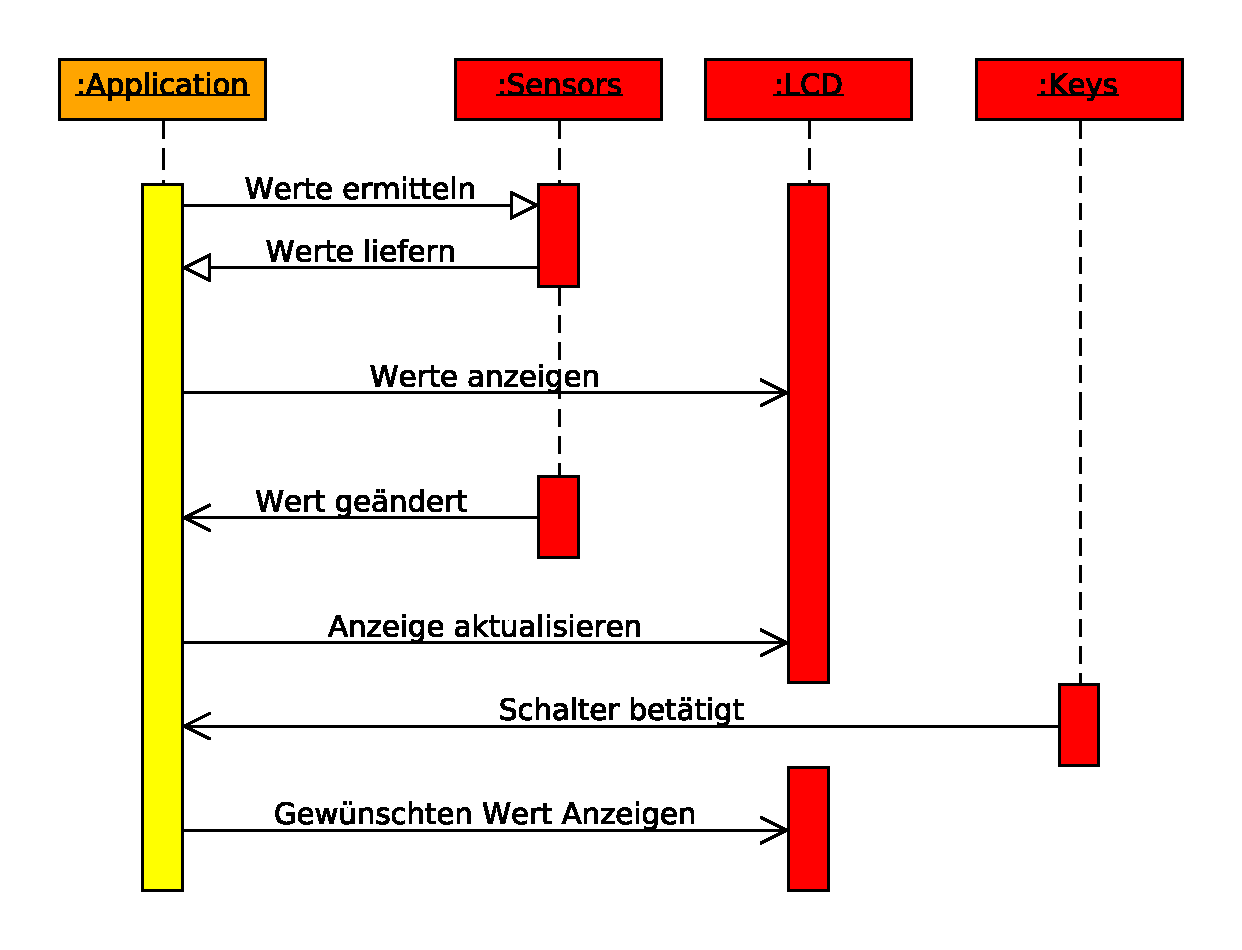
\includegraphics[width=.9\textwidth]{sequence-startup-running}
    \caption{Die Anwendung reagiert auf Änderungen der Messwerte und auf Tastendruck}
    \label{fig:sequence-startup-running}
\end{figure}

\begin{figure}[ht]
    \centering
    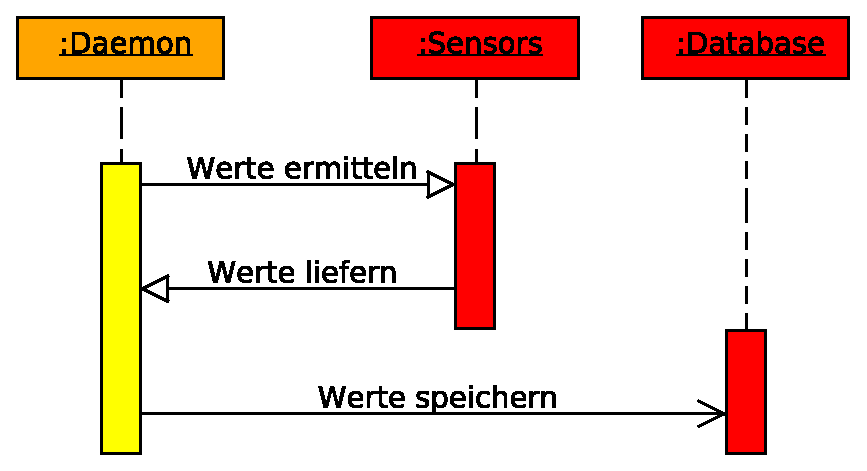
\includegraphics[width=.7\textwidth]{sequence-store-periodic}
    \caption{Die Messwerte werden periodisch mittels Polling gespeichert}
    \label{fig:sequence-store-periodic}
\end{figure}

\section{Synthese}

\subsection{Abstraktionen}
Somit ergeben sich die folgenden Abstraktionen mit ihren Eigenschaften und Methoden:

\begin{itemize}
    \item Sensoren
        \begin{itemize}
            \item Alle Sensoren bieten die Möglichkeit, den aktuellen Messwert zu
                ermitteln und einen Beobachter zu benachrichtigen, sobald der aktuelle Wert
                signifikant~\footnote{Mit signifikant ist gemeint, dass sich der Wert mind. soweit
                geändert hat, als dass die Änderung auf dem Display erkennbar ist.}.
                Folgende Sensoren werden benötigt:
                \begin{itemize}
                    \item Temperatur-Sensor
                    \item Feuchtigkeit-Sensor
                    \item Luftdruck-Sensor
                    \item Licht-Sensor
                \end{itemize}
        \end{itemize}
    \item Datenbank
        \begin{itemize}
            \item Die Datenbank muss eine Menge von Messwerten (Temperatur, Luftdruck
                etc.) mit dem aktuellen Zeit Stempel speichern.
        \end{itemize}
    \item LCD
        \begin{itemize}
            \item Das Display muss die folgenden Elemente darstellen können:
                \begin{itemize}
                    \item Die aktuellen Messwerte
                    \item Die IP Adresse des Gerätes
                    \item Eine Fehlermeldung
                \end{itemize}
        \end{itemize}
    \item Schalter
        \begin{itemize}
            \item Der Schalter bietet die Möglichkeit, einen Beobachter zu registrieren,
                welcher nach dem Betätigen des Schalters benachrichtigt wird.
        \end{itemize}
\end{itemize}

\subsection{Struktur}
% Die Anwendung befindet sich im laufenden Zustand, sobald das Gerät gestartet wird. Sie
% wird bis zum Herunterfahren des Gerätes nicht mehr gestoppt. Es handelt sich also um einen
% Dämon, welcher über geeignete Massnahmen dazu bewegt werden muss, die Werte auszulesen,
% diese zu speichern und auf dem Display anzuzeigen. Zudem kann der Anwender die Anzeige auf
% dem Display wechseln, resp. er kann den anzuzeigenden Wert wählen oder die IP Adresse
% anzeigen lassen.

% Das Auslesen und Abspeichern der Werte läuft vollkommen automatisch im Hintergrund ab,
% diesen Vorgang kann der Benutzer nicht beeinflussen. Daher kann dies in einem eigenen
% Thread abgearbeitet werden, welcher während der gesamten Laufzeit des Dämons aktiv ist.
% Für den Wechsel der Anzeige muss der Dämon resp. die zugehörige Einheit auf Tastendruck
% und auf Änderungen des angezeigten Wertes reagieren.

Statt einen monolithischen Ansatz zu verfolgen und dem LCD die Rolle der View zu
zuordnen, sollte eher angestrebt werden, einen modularen Aufbau zu erzielen. Da
andernfalls das Hinzufügen von weiteren Sensoren und die Implementierung der View
schwierig sind. Eine einfache Indirektion löst dieses Problem: Statt dass die View auf
alle Sensoren lauscht, existiert zu jedem Sensor eine kleine View, welche nur auf einen
einzelnen Sensor lauscht und das LCD als Zeichen-Oberfläche erhält. Auf diese Weise können
die einzelnen Sensoren leichter ausgetauscht werden und die Anwendung weist eine
schwächere Kopplung auf.

Zusammenfassend ergibt sich die Klassenstruktur wie sie in Abbildung
\ref{fig:class-diagram} dargestellt ist.

\begin{figure}[ht]
    \centering
    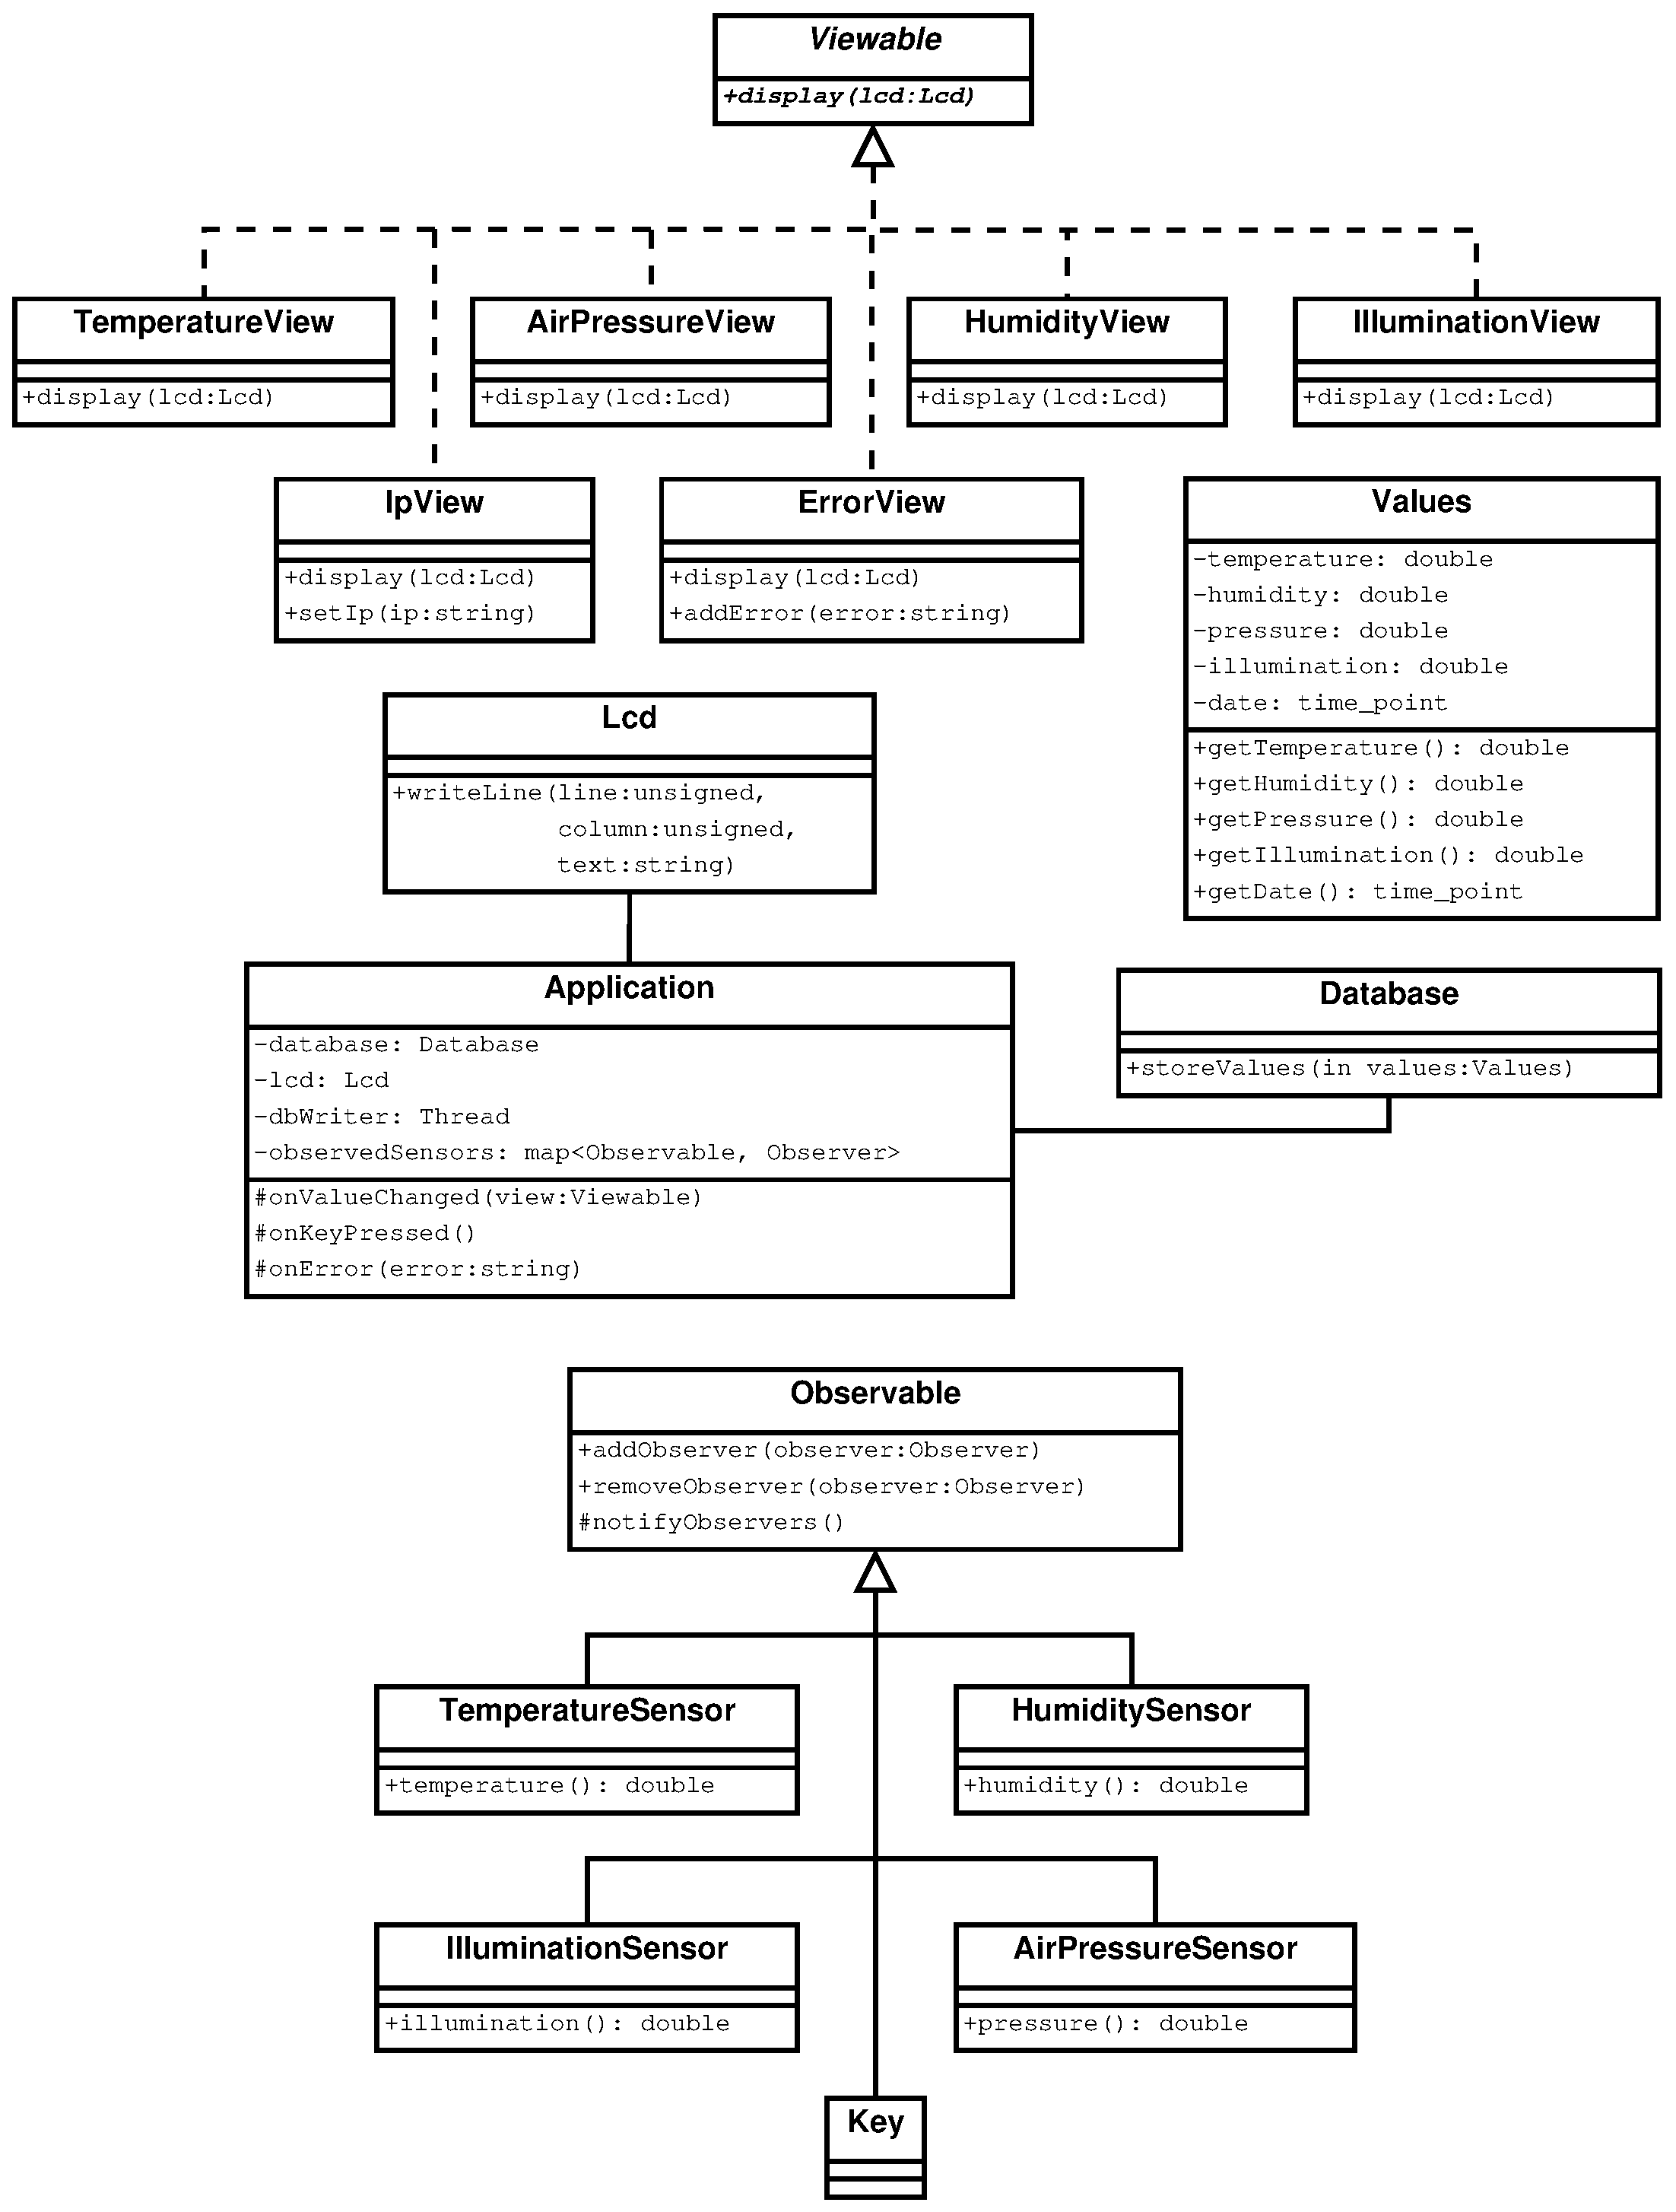
\includegraphics[width=\textwidth]{class-diagram}
    \caption{Klassen Diagramm}
    \label{fig:class-diagram}
\end{figure}

Der Grund, weswegen keine Schnittstelle Observer definiert wurde, liegt darin, dass mit
C++ gearbeitet wird und statt einer Schnittstelle für den Observer lediglich ein
Funktionsobjekt verwendet werden kann. Da der Funktor vorgängig mit Argumenten gebunden
werden kann, muss dem Observer beim Aufruf kein spezifisches Argument mitgegeben werden.
Generell interessiert den Beobachter lediglich, dass sich der Wert des beobachteten
Sensors geändert hat. Eine Schnittstelle des Beobachters, welche beispielsweise den Sensor
als Argument erhält, wäre nutzlos, da es sich bei dem Sensor, welcher der Observer
erhalten würde, um eine Schnittstelle handeln würde, um den konkreten Sensor zu erhalten,
wäre daher ein casting notwendig. Dies entfällt durch das vorgängige Binden des Funktors,
beispielsweise kann eine Instanz einer \texttt{std::function<void()>} mittels einer
Closure oder einer gebundenen Member Funktion erzeugt werden.

Aus Platzgründen wurden nicht alle Attribute und Methoden der Klasse Application
notiert, generell handelt es sich um eine grobe Sicht auf die Architektur. Eine zentrale
Rolle spielt der Konstruktor der Klasse, darin werden die Views bei den Sensoren als
Beobachter registriert und die Anzeige mit den aktuellen Werten versehen. Bei einem
Wechsel der Anzeige können schliesslich die registrierten Beobachter de-registriert werden
um die IP Adresse oder im Fehlerfall die Fehlermeldung anzuzeigen. Eine Alternative zu dem
erwähnten Modell, in welchem die Views auf Änderungen am Modell lauschen, besteht darin,
dass nicht die Views direkt auf Änderungen am Display lauschen sondern
Application. Dies kann realisiert werden, indem wie angedeutet, eine Methode
\texttt{onValueChanged} als Grundlage dient, einen Observer zu erstellen. Die Methode kann
mit \texttt{this} und der zugehörigen View gebunden werden, um einen Funktor zu erzeugen,
welcher als Beobachter eines Sensores dient. Analog dazu muss schliesslich noch dasselbe
für den Thread \texttt{dbWriter} getan werden, indem statt bloss den Observer mit dem
Sensor zu speichern, zusätzlich noch ein Funktor gespeichert wird, welcher den zugehörigen
Wert in Values setzt. Schliesslich kann der Thread die map durchwandern, jeden zugehörigen
Funktor mit einem Value aufrufen, den Zeit Stempel setzen und die so assemblierten Werte
mittels der Datenbank speichern. Im Falle eines Wechsels der Anzeige werden jeweils die
Beobachter bei den Sensoren an- resp. abgemeldet.

\section{Qualitätssicherung}
Um den notwendigen Qualität Standard zu ermitteln, werden die funktionalen Anforderungen
herbeigezogen um daraus entsprechende Test Szenarien abzuleiten.

\begin{itemize}
    \item Luftdruck, Temperatur, Feuchtigkeit und Lichtstärke müssen korrekt ermittelt,
        dargestellt und gespeichert werden.
        \begin{itemize}
            \item Mittels manuellen Tests und einem Referenz Gerät kann verifiziert
                werden, ob die Werte in einem gültigen Toleranzbereich liegen. Falls dies
                über das LCD verifiziert werden kann, ist auch sichergestellt, dass die
                Werte entsprechend ermittelt werden.
            \item Mittels manueller Überprüfung kann verifiziert werden, ob der
                entsprechende Inhalt in der Datenbank abgelegt wurde. Beispielsweise
                mittels einer SQLite Shell.
        \end{itemize}
    \item Sämtliche Informationen müssen über eine Web Applikation eingesehen werden
        können.
        \begin{itemize}
            \item Auch dies kann mittels manueller Überprüfung auf dieselbe Weise
                verifiziert werden: Sämtliche online dargestellten Werte müssen im
                Vergleich mit den Werten eines Referenz Gerätes in einem gültigen
                Toleranzbereich liegen. Zudem kann überprüft werden, ob zuvor gespeicherte
                Daten abrufbar sind.
        \end{itemize}
\end{itemize}

Zudem müssen weitere Risiken berücksichtigt werden, wobei externe Fehlerquellen wie ein
Ausfall der Stromzufuhr ignoriert werden, solche Fehler können nicht adressiert werden.
Ein Ausfall des LCD oder ein festsitzender Schalter können ebenfalls nicht behandelt
werden. Es sollte jedoch sichergestellt werden, dass keine falschen Werte gespeichert
werden, falls ein Sensor ausfällt, sollte dies von der Anwendung erkannt werden.

Zudem ist es möglich, dass irgendwann der Speicher ausgeht. Es wäre auch denkbar, dass
eine sehr grosse Datenbank Probleme verursacht.

Es bleiben zusätzlich die folgenden möglichen Fehler, welche behandelt werden müssen:

\begin{itemize}
    \item Ausfall von Sensoren
        \begin{itemize}
            \item Im Falle von ausgefallenen Sensoren sollen die entsprechenden Werte
                nicht gespeichert werden. Auf dem LCD soll in diesem Fall eine
                entsprechende Fehlermeldung angezeigt werden.
        \end{itemize}
    \item Kein Speicherplatz mehr verfügbar
        \begin{itemize}
            \item Falls das Speichern der Messwerte fehlschlägt, weil kein Speicherplatz
                mehr verfügbar ist, soll auf dem LCD ebenfalls eine entsprechende
                Fehlermeldung angezeigt werden.
        \end{itemize}
    \item Kein Netzwerk verfügbar
        \begin{itemize}
            \item In diesem Fall soll bei einem Wechsel der Anzeige zur IP Adresse eine
                Fehlermeldung angezeigt werden.
        \end{itemize}
\end{itemize}

\section{Testing}

Um den korrekten Betrieb des Systems zu verifizieren, werden Testfälle definiert, welche
im Anschluss an die Implementierung und auch währenddessen durchlaufen werden. Die
benötigten Testfälle können anhand der zuvor ermittelten Kriterien und Risiken erstellt
werden.

\subsection{TC1 - Ermitteln der Werte}
Das korrekte Ermitteln der Werte der Sensoren wird wie beschrieben manuell überprüft. Ein
Referenz Gerät liefert die Werte, mit welchen die ermittelten Werte verglichen werden.
Die Differenz muss anschliessend im gültigen Toleranzbereich liegen.

\subsection{TC2 - Speicherung}
Mittels einer SQLite Shell wird geprüft, ob der periodisch gespeicherte Inhalt in der
Datenbank vorhanden ist.

\subsection{TC3 - Aktuelle Daten über die Web Applikation}
Mittels manuellem Testing wird verifiziert, dass die von der Web Applikation dargestellten
Werte im gültigen Toleranzbereich liegen.

\subsection{TC4 - Gespeicherte Daten über die Web Applikation}
Mittels manuellem Testing wird verifiziert, dass die zuvor gespeicherten Werte verfügbar
sind.

\subsection{TC5 - Ausfall aller Sensoren}
Während des Betriebs wird das Verbindungskabel zwischen dem Raspberry Pi und der
Wetterstation getrennt. Auf der Anzeige der Werte der Sensoren muss eine entsprechende
Fehlermeldung angezeigt werden.

\subsection{TC6 - Speicherplatz}
Es wird eine ausreichend grosse Datei auf eine separate, für diesen Test präparierte SD
Karte gelegt. Die Datei muss so gross sein, dass bloss noch wenige Bytes an Speicher auf
der Karte vorhanden sind. Eine solche Datei kann mittels \texttt{dd} erstellt werden.
Anschliessend wird verifiziert, dass die Anwendung versucht, die Datensätze abzulegen.
Sobald dies fehlschlägt, muss eine entsprechende Fehlermeldung angezeigt werden.


% \FloatBarrier
% \appendix

% \listoftables
\listoffigures
% \lstlistoflistings
% \printglossary[title = Glossar, toctitle = Glossar]

\bibliographystyle{apacite}
\bibliography{02-software-on-pi}

\end{document}
